% !TeX program = pdflatex
% Build: latexmk -pdf -interaction=nonstopmode -halt-on-error main.tex
% Optional presenter copy: define \PresenterNotes before inputting this file.
\documentclass[aspectratio=169,11pt]{beamer}
\usepackage[T1]{fontenc}
\usepackage{lmodern}
\usepackage{amsmath,amssymb,mathtools,bm}
\usepackage{booktabs,tabularx,array}
\usepackage{graphicx,microtype,xurl}
\usepackage{pgfplots,pgfpages,listings}
\pgfplotsset{compat=1.18}
\usefonttheme{professionalfonts}
\definecolor{ink}{HTML}{17324D}
\definecolor{bodyink}{HTML}{263747}
\definecolor{accent}{HTML}{087F8C}
\definecolor{warm}{HTML}{B45C29}
\definecolor{rulegray}{HTML}{D6DFE7}
\definecolor{muted}{HTML}{56697A}
\setbeamercolor{normal text}{fg=bodyink,bg=white}
\setbeamercolor{structure}{fg=ink}
\setbeamercolor{title}{fg=ink}
\setbeamercolor{subtitle}{fg=muted}
\setbeamercolor{frametitle}{fg=ink,bg=white}
\setbeamercolor{alerted text}{fg=accent}
\setbeamercolor{itemize item}{fg=accent}
\setbeamercolor{enumerate item}{fg=accent}
\setbeamercolor{footline}{fg=muted,bg=white}
\setbeamerfont{title}{size=\fontsize{29}{34}\selectfont,series=\bfseries}
\setbeamerfont{subtitle}{size=\fontsize{14}{18}\selectfont}
\setbeamerfont{frametitle}{size=\fontsize{18}{22}\selectfont,series=\bfseries}
\setbeamerfont{footline}{size=\fontsize{7}{9}\selectfont}
\setbeamersize{text margin left=9mm,text margin right=9mm}
\setbeamertemplate{navigation symbols}{}
\setbeamertemplate{bibliography item}{}
\setbeamertemplate{itemize item}{\raise0.15ex\hbox{\scriptsize\(\bullet\)}}
\setbeamertemplate{frametitle}{%
  \vspace{2mm}\insertframetitle\par\vspace{1.5mm}%
  {\color{rulegray}\hrule height0.5pt}\vspace{1.3mm}}
\setbeamertemplate{footline}{%
  \leavevmode\hbox{\begin{beamercolorbox}[wd=\paperwidth,ht=3.3mm,dp=1.3mm,
    leftskip=9mm,rightskip=9mm]{footline}%
    \usebeamerfont{footline}The Transformer\hfill
    \insertframenumber\,/\,\inserttotalframenumber
  \end{beamercolorbox}}}
\ifdefined\PresenterNotes
  \setbeameroption{show notes on second screen=right}
\else
  \setbeameroption{hide notes}
\fi
\hypersetup{pdftitle={The Transformer: Architecture, Mathematics, and Computation},
  pdfsubject={General Transformer architecture lecture},
  colorlinks=true,urlcolor=accent,linkcolor=ink}
\pdfstringdefDisableCommands{\def\translate#1{#1}}
\newcolumntype{Y}{>{\raggedright\arraybackslash}X}
\setlength{\emergencystretch}{2em}
\setlength{\parskip}{0.25em}
\setlength{\abovedisplayskip}{5pt}
\setlength{\belowdisplayskip}{5pt}
\renewcommand{\arraystretch}{1.18}
\newcommand{\R}{\mathbb{R}}
\newcommand{\E}{\mathbb{E}}
\newcommand{\one}{\mathbf{1}}
\newcommand{\T}{\mathsf{T}}
\newcommand{\lead}[1]{{\color{ink}\bfseries #1}\par\vspace{1.2mm}}
\newcommand{\src}[1]{\par\vfill{\fontsize{7}{8.5}\selectfont\color{muted}#1}\par}
\newcommand{\paper}{\href{https://arxiv.org/abs/1706.03762}{Vaswani et al.\ (2017)}}
\newcommand{\code}[1]{\texttt{\detokenize{#1}}}
\DeclareMathOperator{\softmax}{softmax}
\DeclareMathOperator{\Att}{Att}
\DeclareMathOperator{\MHA}{MHA}
\DeclareMathOperator{\FFN}{FFN}
\DeclareMathOperator{\LN}{LN}
\DeclareMathOperator{\Concat}{Concat}
\DeclareMathOperator{\Var}{Var}
\DeclareMathOperator{\diag}{diag}
\DeclareMathOperator*{\argmax}{arg\,max}
\lstset{basicstyle=\ttfamily\fontsize{9}{11}\selectfont,
  columns=fullflexible,keepspaces=true,showstringspaces=false,
  breaklines=true,frame=none,aboveskip=1.5mm,belowskip=1.5mm,
  keywordstyle=\color{accent}\bfseries,commentstyle=\color{muted}}
\title{The Transformer}
\subtitle{Architecture, mathematics, and computation}
\author{}
\date{}
\begin{document}

% 01
\begin{frame}[plain]
  \vspace{8mm}\titlepage\vspace{-9mm}
  \begin{center}
    \large Attention as a learned rule for exchanging information
  \end{center}
  \vfill
  {\small\color{muted}Foundations in \emph{Attention Is All You Need} (2017)}
  \note{The main construction is the original encoder--decoder Transformer
  with post-layer normalization. Later variants are labeled explicitly.
  The intended audience knows matrix multiplication, derivatives, and
  elementary probability. Token states are row vectors throughout.}
\end{frame}

\section{Problem and representation}
% 02
\begin{frame}[t]{Learning objectives}
\lead{A complete forward pass, with the dimensions visible}
\begin{enumerate}
  \item Represent tokens and their positions as vectors.
  \item Compute one attention head, then combine several heads.
  \item Assemble the encoder, decoder, and output distribution.
  \item Relate training, generation, and computational cost.
\end{enumerate}
\vspace{2mm}
The main lecture uses the original 2017 architecture. Appendices give
derivations, parameter counts, and exercises with solutions.
\src{Prerequisites: basic linear algebra, probability, and differentiation.}
\note{Allow about 50--60 minutes for the main lecture, depending on how
much of the example the audience calculates. Select appendices for questions.
Tokenization algorithms and optimizer implementation are outside the
main derivation.}
\end{frame}

% 03
\begin{frame}[t]{The sequence modeling problem}
Let $\mathcal V_s$ and $\mathcal V_t$ be source and target vocabularies.
For source $x=(x_1,\ldots,x_n)$ and target $y=(y_1,\ldots,y_m)$,
\[
  p_\theta(y\mid x)=\prod_{t=1}^{m}p_\theta(y_t\mid y_{<t},x),
  \qquad y_{<t}=(y_1,\ldots,y_{t-1}).
\]
\begin{itemize}
  \item $x_i\in\mathcal V_s$, $y_t\in\mathcal V_t$, and $n,m\geq1$.
  \item $\theta$ denotes all learned parameters.
  \item $y_m=\texttt{EOS}$ marks the end of the target sequence.
  \item A separate $y_0=\texttt{BOS}$ starts the decoder input.
\end{itemize}
The encoder represents $x$. The decoder models each conditional factor.
\src{\paper, Sections 1 and 3. EOS is included in the modeled target length.}
\note{The factorization is the probability chain rule, with the model
parameterizing its factors. For t=1 the target prefix is empty. BOS is an
input convention and is not an additional predicted token in this notation.
The likelihood applies to a finite target ending in EOS. A maximum generation
length can be imposed operationally.}
\end{frame}

% 04
\begin{frame}[t]{Recurrence and direct token interaction}
\begin{columns}[T,onlytextwidth]
\begin{column}{0.46\textwidth}
  \lead{A recurrent layer}
  \[h_i=f_\theta(h_{i-1},e_i).\]
  $e_i$ is token $i$'s input vector. Computing $h_i$ requires the previous
  state $h_{i-1}$.
  \par\vspace{2mm}
  A dependency across the sequence can pass through $O(n)$ recurrent steps.
\end{column}
\begin{column}{0.49\textwidth}
  \lead{A self-attention layer}
  \[o_i=\sum_{j=1}^{n}a_{ij}(H)\,v_j.\]
  $H$ contains the input token states. The layer learns the weights
  $a_{ij}(H)$ from those states.
  \par\vspace{2mm}
  An allowed token can contribute directly to another token in one layer.
\end{column}
\end{columns}
\src{\paper, Sections 1 and 4. Generation still has sequential target steps.}
\note{The recurrent equation assumes an initial state $h_0$. This compares
dependencies within a layer and paths between positions. It does not prove
that attention is faster for every sequence length or hardware configuration.
Projections and feed-forward layers also have costs. A direct interaction
exists only where the attention mask permits it.}
\end{frame}

% 05
\begin{frame}[t]{The original encoder--decoder architecture}
\begin{columns}[T,onlytextwidth]
\begin{column}{0.43\textwidth}
  \centering
  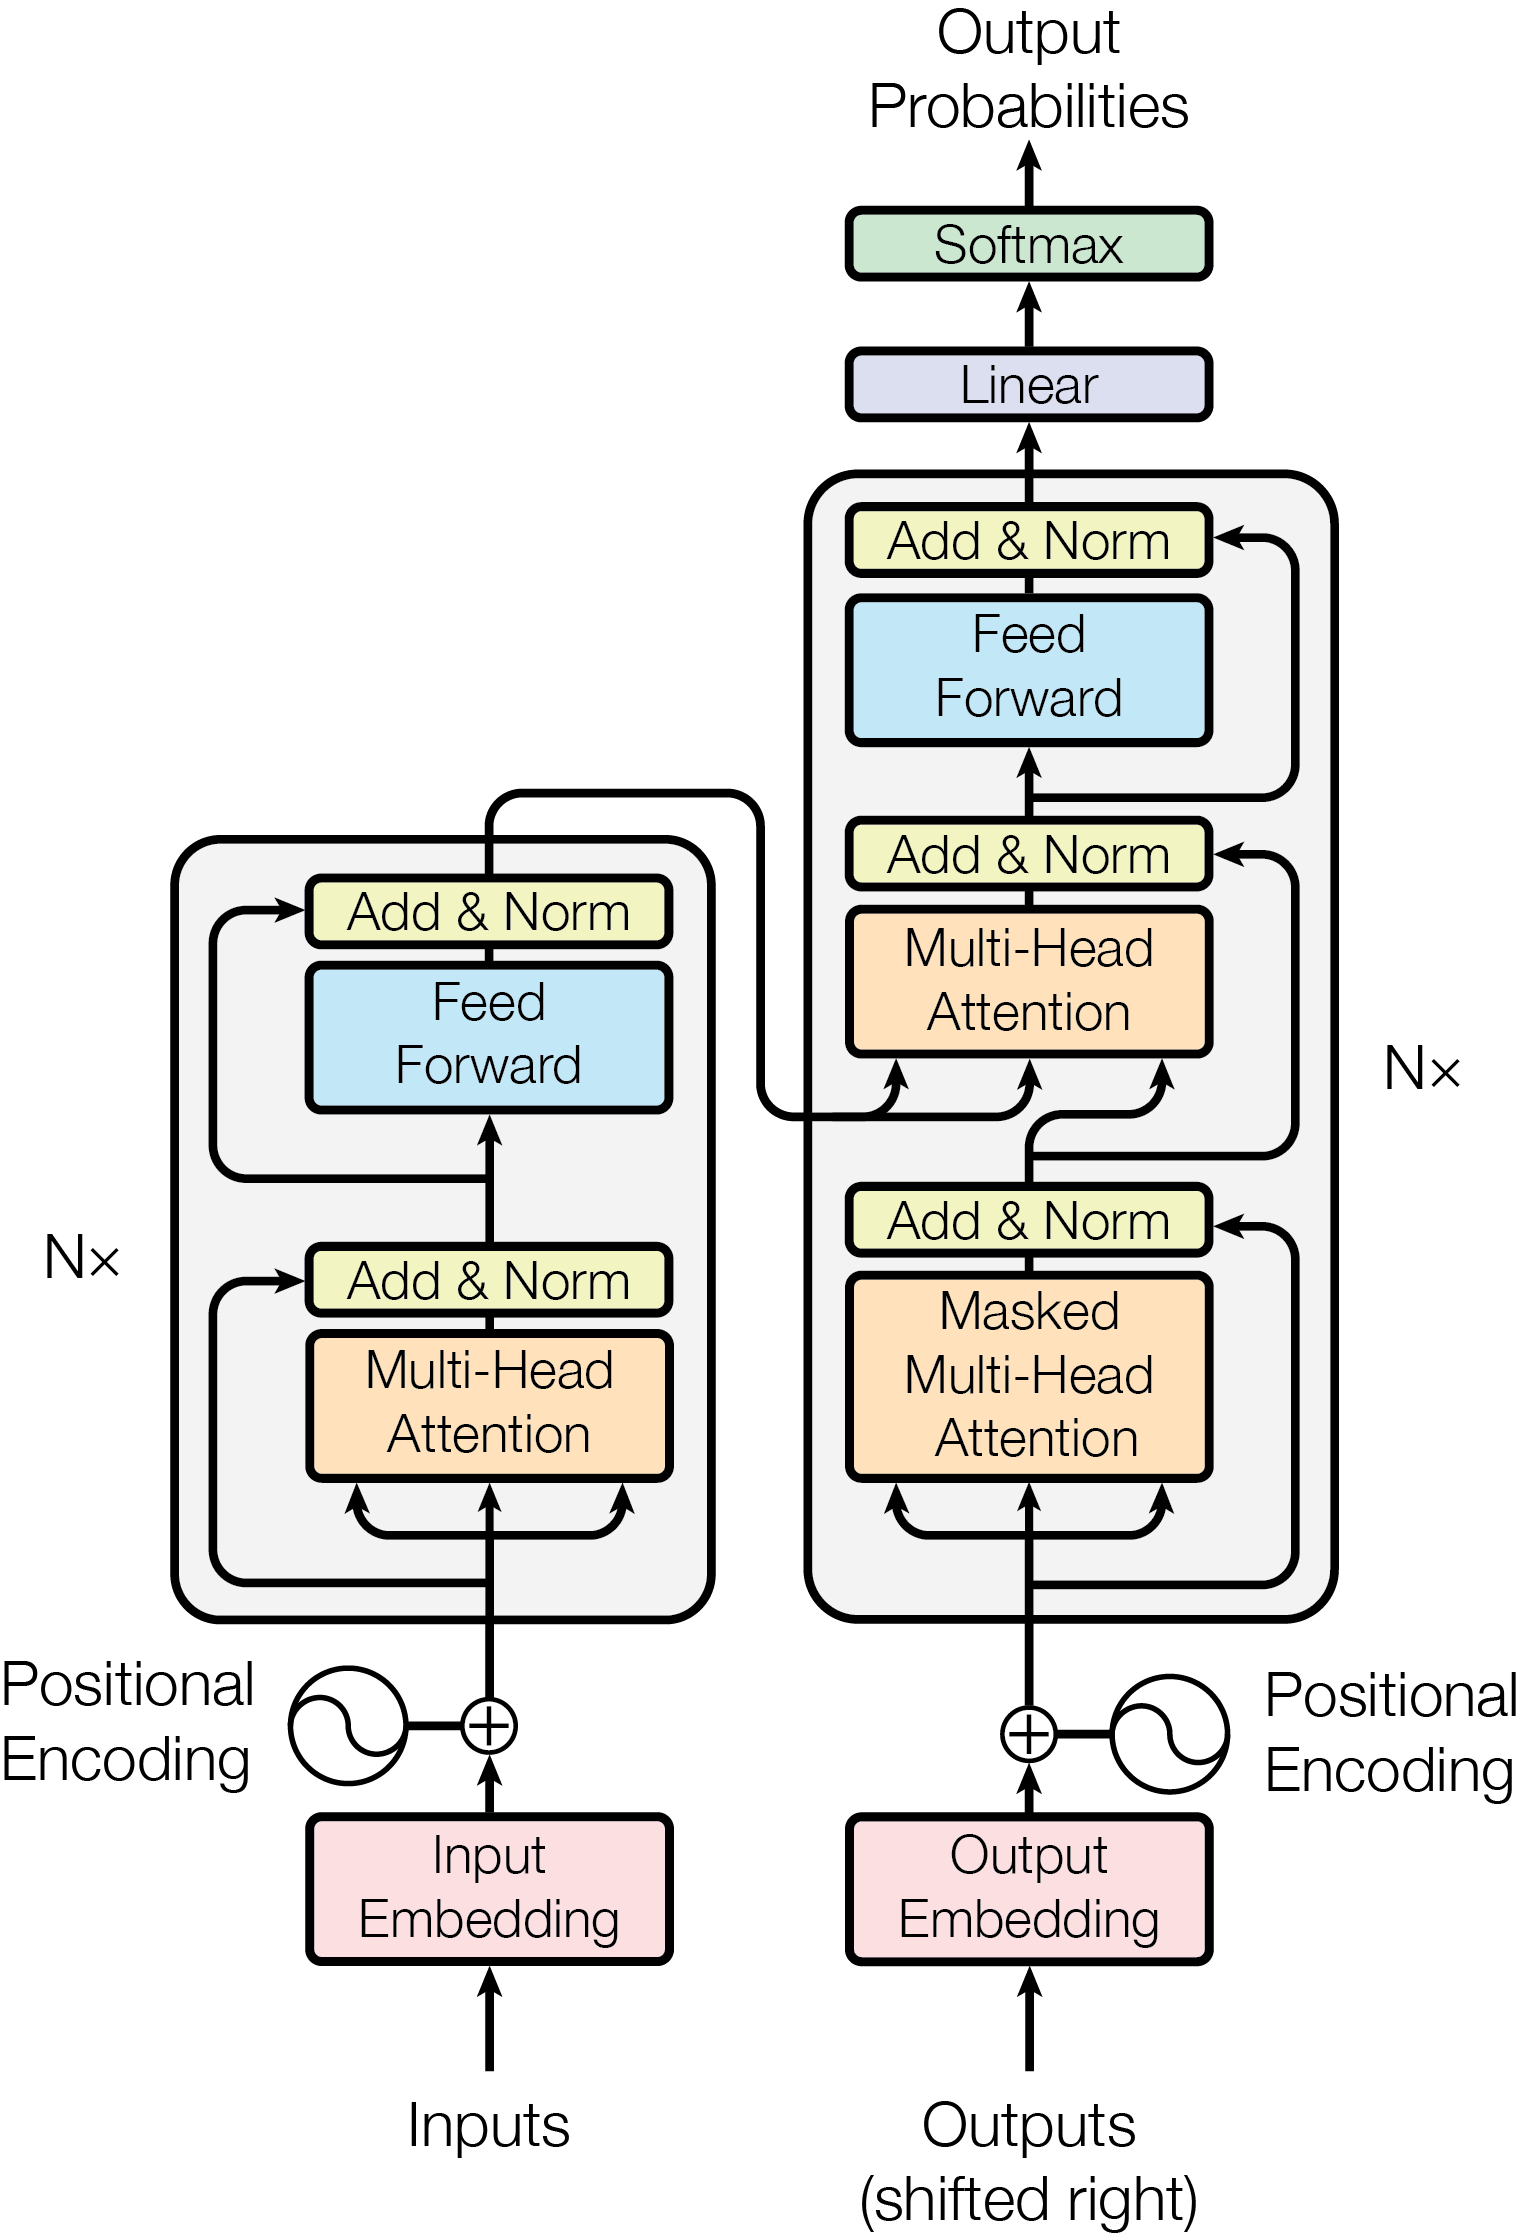
\includegraphics[height=61mm,keepaspectratio]{images/transformer_original.png}
\end{column}
\begin{column}{0.54\textwidth}
  \lead{Encoder}
  Source embeddings and positions enter repeated self-attention and
  feed-forward blocks.
  \par\vspace{2mm}
  \lead{Decoder}
  Shifted target embeddings enter masked self-attention, attention over
  encoder states, and feed-forward blocks.
  \par\vspace{2mm}
  A linear map and softmax produce a distribution over the target vocabulary.
  \par\vspace{1mm}
  In the base model, each stack contains six layers.
\end{column}
\end{columns}
\src{Figure 1 reproduced from \paper, \emph{Attention Is All You Need}.}
\note{Trace the source sequence up the left stack. Its output supplies
keys and values to every decoder cross-attention sublayer. Each such
sublayer learns its own projections. Repeated layers share their pattern
but have distinct parameters. Add and Norm means residual addition followed
by layer normalization in the original architecture.}
\end{frame}

% 06
\begin{frame}[t]{Notation and conventions}
\small
\begin{tabularx}{\textwidth}{@{}lX@{}}
\toprule
Symbol & Meaning \\
\midrule
$n,m$ & Source length and target length, including target EOS \\
$d$ & Model width, also written $d_{\mathrm{model}}$ \\
$h$ & Number of attention heads \\
$L_e,L_d$ & Numbers of encoder layers and decoder layers \\
$d_k,d_v$ & Key/query width and value width of one head \\
$d_{\mathrm{ff}}$ & Hidden width of the feed-forward network \\
$v_s,v_t$ & Vocabulary sizes $|\mathcal V_s|$ and $|\mathcal V_t|$ \\
$H\in\R^{n\times d}$ & One source token state in each row \\
$S\in\R^{m\times d}$ & One decoder token state in each row \\
$\one_r\in\R^{r\times1}$ & Column vector of ones for broadcasting row biases \\
\bottomrule
\end{tabularx}
\src{Sequence indices start at 1. Position-encoding coordinates start at 0. Batch axes are initially omitted.}
\note{All dimensions are positive integers. Token vectors are rows.
A superscript T means transpose. Superscripts in parentheses are layer
indices, not powers. Operator parameters are distinct between layers and
sublayers even when an operator name repeats.}
\end{frame}

% 07
\begin{frame}[t]{Token embeddings and initial states}
Learn $E_s\in\R^{v_s\times d}$ and $E_t\in\R^{v_t\times d}$.
Their rows are embedding vectors indexed by token IDs.
\[
\begin{aligned}
 H^{(0)}_{i,:}&=\sqrt d\,E_s[x_i,:]+P_{i-1,:}, &&1\leq i\leq n,\\
 S^{(0)}_{t,:}&=\sqrt d\,E_t[y_{t-1},:]+P_{t-1,:}, &&1\leq t\leq m.
\end{aligned}
\]
\begin{itemize}
  \item $P_{p,:}\in\R^{1\times d}$ describes zero-based position $p$.
  \item Both sums have width $d$, so residual connections preserve shape.
  \item Decoder row $t$ starts with the previous target token $y_{t-1}$.
\end{itemize}
\src{\paper, Sections 3.4--3.5. These equations omit embedding dropout.}
\note{The vocabularies include required special tokens. $E_s[x_i,:]$ means
the row assigned to token $x_i$. The positional rule can be evaluated for
different source and target lengths. The original model also applies
dropout to these sums. Embedding/output weight tying requires compatible
vocabularies and is discussed with the output projection.}
\end{frame}

% 08
\begin{frame}[t]{Order and permutation equivariance}
Let $\Pi\in\R^{n\times n}$ be a permutation matrix, which reorders rows.
Let $F$ be unmasked self-attention without positional information. Then
\[F(\Pi H)=\Pi F(H).\]
This property is \alert{permutation equivariance}: reordering the input
reorders the output in the same way.
\begin{itemize}
  \item Token identities alone do not specify their absolute positions.
  \item Adding a position vector assigns a different input to each position.
  \item A fixed causal mask also encodes an ordering constraint.
\end{itemize}
\src{Algebraic derivation in Appendix B. The statement excludes fixed order-dependent masks or biases.}
\note{Equivariance differs from invariance: the output changes by the
same permutation rather than staying identical. Shared row-wise affine
maps, layer normalization, and feed-forward networks preserve this
property in deterministic evaluation. Independent dropout masks do not
necessarily preserve exact samplewise equivariance during training.}
\end{frame}

% 09
\begin{frame}[t]{Sinusoidal positional encoding}
\begin{columns}[T,onlytextwidth]
\begin{column}{0.52\textwidth}
  For even $d$ and $0\leq r<d/2$, define
  \[\omega_r=10000^{-2r/d}.\]
  At position $p\in\{0,1,2,\ldots\}$,
  \[
  \begin{aligned}
    P_{p,2r}&=\sin(p\omega_r),\\
    P_{p,2r+1}&=\cos(p\omega_r).
  \end{aligned}
  \]
  Each pair uses a different frequency.
  A fixed offset acts by a rotation within each pair.
\end{column}
\begin{column}{0.45\textwidth}
  \centering
  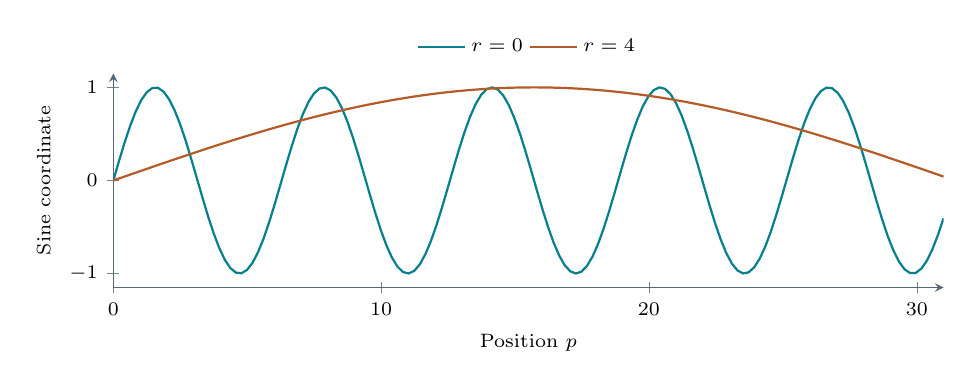
\begin{tikzpicture}
  \begin{axis}[width=\linewidth,height=43mm,
    xmin=0,xmax=31,ymin=-1.15,ymax=1.15,
    xlabel={Position $p$},ylabel={Sine coordinate},
    xtick={0,10,20,30},ytick={-1,0,1},
    tick label style={font=\scriptsize},label style={font=\scriptsize},
    axis lines=left,axis line style={muted},
    legend style={font=\scriptsize,draw=none,at={(0.5,1.03)},anchor=south,legend columns=2},
    domain=0:31,samples=150]
    \addplot[accent,thick] {sin(deg(x))};
    \addlegendentry{$r=0$}
    \addplot[warm,thick] {sin(deg(x/10))};
    \addlegendentry{$r=4$}
  \end{axis}
  \end{tikzpicture}
  {\scriptsize Illustrative width $d=32$}
\end{column}
\end{columns}
\src{\paper, Section 3.5. Appendix C derives the offset identity. Longer-length accuracy needs evaluation.}
\note{The coordinate indices 2r and 2r+1 are zero-based. The plotted
curves use $d=32$, so $\omega_0=1$ and $\omega_4=0.1$. This is a function plot,
not empirical data. Position vectors remain defined beyond training
lengths, but useful prediction there is an empirical question. Learned
absolute embeddings and other position mechanisms are alternatives.}
\end{frame}

\section{Attention}
% 10
\begin{frame}[t]{Queries, keys, and values}
For one query row $q\in\R^{1\times d_k}$, let
$k_j\in\R^{1\times d_k}$ and $v_j\in\R^{1\times d_v}$ be key/value pairs.
\[
  s_j=\frac{qk_j^{\T}}{\sqrt{d_k}},\quad
  a_j=\frac{e^{s_j}}{\sum_{r=1}^{n_k}e^{s_r}},\quad
  o=\sum_{j=1}^{n_k}a_jv_j.
\]
\begin{tabularx}{\textwidth}{@{}lX@{}}
\toprule
Query & Determines which keys receive weight \\
Key & Participates in the compatibility score \\
Value & Contributes to the weighted output \\
\bottomrule
\end{tabularx}
\src{\paper, Section 3.2. These are computational roles. Here $n_k\geq1$ and all keys are allowed.}
\note{The scalar $qk_j^{\T}$ is a dot product. A key and a value refer to
the same candidate position but are usually different projections. The
query need not express a natural-language question. Each output has
value width $d_v$. The displayed weights are nonnegative and sum to one.}
\end{frame}

% 11
\begin{frame}[t]{The scale factor in dot-product attention}
Suppose the $2d_k$ scalar components of random rows $q,k$ are mutually
independent, with mean $0$ and variance $1$. Then
\[
  \E[qk^{\T}]=0,\qquad \Var(qk^{\T})=d_k,\qquad
  \Var\!\left(\frac{qk^{\T}}{\sqrt{d_k}}\right)=1.
\]
\begin{itemize}
  \item The root-mean-square unscaled dot product equals $\sqrt{d_k}$
        under these assumptions.
  \item Very different logits can make softmax strongly concentrated.
  \item Scaling controls this dimensional effect in the illustrative model.
\end{itemize}
\src{\paper, Section 3.2.1. Appendix A gives the full variance calculation.}
\note{These probabilistic assumptions motivate the scale factor.
Learned queries and keys need not remain independent or have unit variance.
Self-attention queries and keys can be correlated, especially at the same
position. Softmax saturation can reduce Jacobian entries. Scaling alone
does not guarantee optimization stability.}
\end{frame}

% 12
\begin{frame}[t]{Masked softmax, one row at a time}
Let $s_{ij}$ be query $i$'s score for key $j$. Let $\mathcal A_i$ be its
\alert{nonempty} set of allowed key indices. Define
\[
  a_{ij}=\begin{cases}
    \displaystyle\frac{\exp(s_{ij}-c_i)}
      {\sum_{r\in\mathcal A_i}\exp(s_{ir}-c_i)},& j\in\mathcal A_i,\\[3mm]
    0,&j\notin\mathcal A_i,
  \end{cases}
  \quad c_i=\max_{r\in\mathcal A_i}s_{ir}.
\]
\begin{itemize}
  \item Normalize across \emph{keys}, separately for each query.
  \item Subtracting $c_i$ preserves the weights and avoids large exponentials.
  \item An entirely masked query needs a separate implementation convention.
\end{itemize}
\src{Maximum subtraction preserves the result by canceling the common factor $e^{-c_i}$.}
\note{For finite allowed scores the denominator is positive. The
allowed weights are positive and sum to one. The mathematical operator
is undefined for an empty allowed set. Some software explicitly outputs
zero for such rows. Padded queries can instead use a safe allowed set
and have their outputs ignored. An ordinary softmax over only negative
infinities does not implement either convention by itself.}
\end{frame}

% 13
\begin{frame}[t]{Worked example: scores and weights}
Choose one query, three keys, and $d_k=2$:
\[
  q=\begin{bmatrix}1&0\end{bmatrix},\qquad
  K=\begin{bmatrix}1&0\\0&1\\1&1\end{bmatrix}.
\]
The score row and its softmax are
\[
\begin{aligned}
  s&=qK^{\T}/\sqrt2
    =\begin{bmatrix}1/\sqrt2&0&1/\sqrt2\end{bmatrix},\\[1mm]
  a&=\frac{1}{2e^{1/\sqrt2}+1}
       \begin{bmatrix}e^{1/\sqrt2}&1&e^{1/\sqrt2}\end{bmatrix}\\
   &\approx\begin{bmatrix}0.401112&0.197776&0.401112\end{bmatrix}.
\end{aligned}
\]
\src{Constructed example. All keys are allowed. Keys 1 and 3 receive equal scores for this query.}
\note{Calculate the three dot products. The third key has an additional
second component, but q's second component is zero. The denominator is
approximately 5.05623. These illustrative numbers are independent of any
trained model.}
\end{frame}

% 14
\begin{frame}[t]{Worked example: the weighted output}
Use the same weight row $a$ and choose value width $d_v=2$:
\[V=\begin{bmatrix}1&0\\0&2\\3&1\end{bmatrix}.\]
\[
\begin{aligned}
  o=aV&\approx0.401112\begin{bmatrix}1&0\end{bmatrix}
    +0.197776\begin{bmatrix}0&2\end{bmatrix}\\
   &\quad+0.401112\begin{bmatrix}3&1\end{bmatrix}\\[1mm]
   &\approx\begin{bmatrix}1.604448&0.796664\end{bmatrix}.
\end{aligned}
\]
Each coordinate uses the \emph{same} attention weights.
The result belongs to the convex hull of the value rows.
\src{Constructed example. The convex-hull claim concerns one head before dropout and output projection.}
\note{The first coordinate is $a_1+3a_3$ and the second is $2a_2+a_3$.
The displayed output uses unrounded weights. Nonnegative weights summing
to one prove the convex-hull claim. The learned projection after head
concatenation need not preserve that interpretation in the original space.}
\end{frame}

% 15
\begin{frame}[t]{Attention in matrix form}
For $n_q$ queries and $n_k$ keys, define
\[
 Q\in\R^{n_q\times d_k},\quad K\in\R^{n_k\times d_k},\quad
 V\in\R^{n_k\times d_v},\quad M\in\{0,-\infty\}^{n_q\times n_k}.
\]
The mask has $M_{ij}=0$ for allowed pairs. Every query has an allowed key.
\[
 A=\softmax_{\mathrm{row}}\!\left(\frac{QK^{\T}}{\sqrt{d_k}}+M\right),
 \qquad \Att(Q,K,V;M)=AV.
\]
\[
 QK^{\T}:\ n_q\times n_k,\quad
 A:\ n_q\times n_k,\quad AV:\ n_q\times d_v.
\]
The transpose converts keys into the column axis of the score matrix.
\src{\paper, Equation (1), with an explicit additive mask and row-wise softmax.}
\note{Additive masking is shorthand for normalization over allowed sets.
The key and value matrices have the same row count. Each A row is a
probability vector. M=0 gives unmasked attention. Attention-weight dropout,
if used during training, changes realized row sums and is omitted here.}
\end{frame}

% 16
\begin{frame}[t]{Self-attention and cross-attention}
Let $U\in\R^{n_q\times d}$ provide query states and
$Z\in\R^{n_k\times d}$ provide memory states. For one head,
\[Q=UW^Q,\quad K=ZW^K,\quad V=ZW^V,\]
where $W^Q,W^K\in\R^{d\times d_k}$ and $W^V\in\R^{d\times d_v}$.
\small
\begin{tabularx}{\textwidth}{@{}lccX@{}}
\toprule
Sublayer & $U$ & $Z$ & Allowed keys \\
\midrule
Encoder self-attention & $H$ & $H$ & All valid source positions \\
Decoder self-attention & $S$ & $S$ & Valid target-input positions $j\leq t$ \\
Decoder cross-attention & $S$ & $H$ & All valid source positions \\
\bottomrule
\end{tabularx}
\src{\paper, Section 3.2.3. The core equations omit projection biases.}
\note{Self-attention uses one sequence as the source for all projections.
Q, K, and V generally differ because their parameter matrices differ.
Cross-attention has $n_q=m$ and $n_k=n$. In the decoder, $S$ means the current
sublayer input. Padding keys are excluded in every case.}
\end{frame}

% 17
\begin{frame}[t]{Multi-head attention}
For heads $a=1,\ldots,h$, learn separate projections and compute
\[
\begin{aligned}
 O_a&=\Att(UW_a^Q,ZW_a^K,ZW_a^V;M)
       \in\R^{n_q\times d_v},\\
 \MHA(U,Z;M)&=\Concat(O_1,\ldots,O_h)W^O
       \in\R^{n_q\times d}.
\end{aligned}
\]
\[
 W_a^Q,W_a^K\in\R^{d\times d_k},\quad
 W_a^V\in\R^{d\times d_v},\quad
 W^O\in\R^{(hd_v)\times d}.
\]
\begin{itemize}
  \item Concatenation joins the head outputs along the feature axis.
  \item Each head computes its own attention weights.
  \item The output projection mixes information across heads.
\end{itemize}
\src{\paper, Section 3.2.2. Biases and attention dropout are omitted from this definition.}
\note{U supplies queries and Z supplies keys and values. For
self-attention set Z=U. Head index a is independent of token indices.
The formula does not force heads to use disjoint positions or learn
particular semantic roles. Each layer has its own learned projections.}
\end{frame}

% 18
\begin{frame}[t]{A complete multi-head shape example}
For $n=5$, use the base widths $d=512$, $h=8$, and $d_k=d_v=64$.
\small
\begin{tabularx}{\textwidth}{@{}lcX@{}}
\toprule
Object & Shape & Operation \\
\midrule
Input $H$ & $5\times512$ & Five token states \\
Each $Q_a,K_a,V_a$ & $5\times64$ & Learned projections of $H$ \\
Each attention matrix $A_a$ & $5\times5$ & Row-wise normalized scores \\
Each head output $O_a$ & $5\times64$ & $A_aV_a$ \\
Concatenated outputs & $5\times512$ & Join eight outputs \\
Output matrix $W^O$ & $512\times512$ & Learned mixing across features \\
Final output & $5\times512$ & Same shape as $H$ \\
\bottomrule
\end{tabularx}
\src{\paper, Section 3.2.2. The sequence length five is illustrative.}
\note{A head uses a learned projection of the entire input width.
It is not restricted to taking a fixed slice of the input coordinates.
With $hd_k=hd_v=d$, projection parameter counts remain $4d^2$ when
biases are omitted. Storing h score matrices still introduces an h factor
in the conventional attention memory.}
\end{frame}

% 19
\begin{frame}[t]{Causal masks and padding masks}
\begin{columns}[T,onlytextwidth]
\begin{column}{0.48\textwidth}
\lead{Causal self-attention}
Row $i$ can use columns $j\leq i$.
\[
 M_{\mathrm{causal}}=
 \begin{bmatrix}
  0&-\infty&-\infty&-\infty\\
  0&0&-\infty&-\infty\\
  0&0&0&-\infty\\
  0&0&0&0
 \end{bmatrix}.
\]
Rows index queries.
Columns index keys.
\end{column}
\begin{column}{0.48\textwidth}
\lead{Padding exclusion}
Let $b_j=1$ for a valid key and $b_j=0$ for padding. Define
\[
 (M_{\mathrm{pad}})_{ij}=
 \begin{cases}0,&b_j=1,\\-\infty,&b_j=0.\end{cases}
\]
For decoder self-attention, combine
\[M=M_{\mathrm{causal}}+M_{\mathrm{pad}}.\]
\end{column}
\end{columns}
\src{Masks restrict keys before normalization. Padded query outputs need an explicit handling convention.}
\note{Encoder self-attention and decoder cross-attention exclude padded
source keys. Decoder self-attention additionally uses the causal mask.
Right-padded decoder queries can retain at least BOS as a valid key and
then be omitted from the loss. Other padding arrangements can create
fully masked rows, which need the convention described earlier.}
\end{frame}

% 20
\begin{frame}[t]{The decoder input shift prevents target leakage}
For target $y=(\texttt{I},\texttt{like},\texttt{math},\texttt{EOS})$:
\begin{center}
\begin{tabular}{@{}cccl@{}}
\toprule
Row $t$ & Decoder input & Predicted token & Visible target prefix \\
\midrule
1 & \texttt{BOS} & \texttt{I} & Empty \\
2 & \texttt{I} & \texttt{like} & \texttt{I} \\
3 & \texttt{like} & \texttt{math} & \texttt{I like} \\
4 & \texttt{math} & \texttt{EOS} & \texttt{I like math} \\
\bottomrule
\end{tabular}
\end{center}
\[S^{(L_d)}_{t,:}\text{ can depend on }x\text{ and }y_{<t}.\]
The causal mask permits diagonal attention because row $t$ contains
$y_{t-1}$. The token being predicted is $y_t$.
\src{\paper, Section 3.1. The shift and causal mask act together.}
\note{By induction over decoder layers, row t depends only on decoder
input rows 1 through t and on encoder states. Row-wise normalization and
feed-forward operations cannot introduce future information. Cross-attention
uses only the source. Without shifting, the diagonal can directly expose
the token whose probability is being trained.}
\end{frame}

\section{Transformer blocks}
% 21
\begin{frame}[t]{The position-wise feed-forward network}
For $H\in\R^{n\times d}$, define
\[
 \FFN(H)=\operatorname{ReLU}(HW_1+\one_n b_1)W_2+\one_n b_2,
\]
where
\[
\begin{aligned}
 W_1&\in\R^{d\times d_{\mathrm{ff}}},&b_1&\in\R^{1\times d_{\mathrm{ff}}},\\
 W_2&\in\R^{d_{\mathrm{ff}}\times d},&b_2&\in\R^{1\times d}.
\end{aligned}
\]
\begin{itemize}
  \item $\operatorname{ReLU}(z)=\max(0,z)$ acts on each entry.
  \item Every token uses the same matrices within a layer.
  \item Different layers have different parameters.
  \item The output has shape $n\times d$.
\end{itemize}
\src{\paper, Section 3.3. The base model has $d=512$ and $d_{\mathrm{ff}}=2048$.}
\note{Attention mixes information across token positions. The FFN mixes
features separately within each token row. Its nonlinearity prevents the
two affine maps from collapsing to one affine map. More recent models may
replace ReLU or use gated networks. Those choices change the block and
potentially its parameter count.}
\end{frame}

% 22
\begin{frame}[t]{Layer normalization and residual connections}
For one row $u=(u_1,\ldots,u_d)$, define
\[
 \mu(u)=\frac1d\sum_{r=1}^d u_r,\qquad
 \sigma^2(u)=\frac1d\sum_{r=1}^d(u_r-\mu(u))^2,
\]
\[
 \LN(u)=\gamma\odot
 \frac{u-\mu(u)\one_d^{\T}}{\sqrt{\sigma^2(u)+\epsilon}}+\beta.
\]
$\gamma,\beta\in\R^{1\times d}$ are learned, $\epsilon>0$, and $\odot$
means entrywise multiplication. Normalize each token row independently.
\[\text{Original residual sublayer:}\qquad \LN\bigl(H+D(F(H))\bigr).\]
$F$ preserves shape. $D$ denotes dropout during training and identity at evaluation.
\src{\href{https://arxiv.org/abs/1607.06450}{Ba et al.\ (2016)}; \paper, Sections 3.1 and 5.4.}
\note{The variance uses divisor d, not the unbiased sample-variance
divisor d-1. Normalization is over features within one token, not over
the batch or sequence. Each sublayer has its own gamma and beta. Residual
dropout with rate rho in [0,1) multiplies entries by independent Bernoulli
variables of mean 1-rho and divides by 1-rho. At evaluation it is the
identity. With positive epsilon, normalized variance need not be exactly one.}
\end{frame}

% 23
\begin{frame}[t]{One encoder layer, explicitly}
Let $H^{(\ell-1)}\in\R^{n\times d}$ enter encoder layer $\ell$.
The source mask $M_s\in\{0,-\infty\}^{n\times n}$ excludes padding keys.
\[
\begin{aligned}
 U^{(\ell)}&=\LN_{\ell,1}\!\left(
 H^{(\ell-1)}+D\!\left(\MHA_{\ell}
 (H^{(\ell-1)},H^{(\ell-1)};M_s)\right)\right),\\[2mm]
 H^{(\ell)}&=\LN_{\ell,2}\!\left(
 U^{(\ell)}+D\!\left(\FFN_{\ell}(U^{(\ell)})\right)\right).
\end{aligned}
\]
\begin{itemize}
  \item Both outputs retain shape $n\times d$.
  \item Repeat for $\ell=1,\ldots,L_e$, using distinct layer parameters.
  \item The final memory is $H_{\mathrm{enc}}=H^{(L_e)}$.
\end{itemize}
\src{\paper, Section 3.1. These are post-layer-normalization equations.}
\note{The formula is exact for the defined attention core and residual
dropout convention. Optional attention-weight dropout and projection
biases can be incorporated inside MHA without changing these outer
equations. D uses separate random masks at separate calls. The initialization
$H^{(0)}$ includes optional embedding dropout as discussed earlier.}
\end{frame}

% 24
\begin{frame}[t]{One decoder layer, explicitly}
Let $S=S^{(\ell-1)}\in\R^{m\times d}$. Use decoder mask $M_t$ and
source-key mask $M_x\in\{0,-\infty\}^{m\times n}$.
\[
\begin{aligned}
 U&=\LN_{\ell,1}\bigl(S+D(\MHA^{\mathrm{self}}_\ell(S,S;M_t))\bigr),\\[2mm]
 R&=\LN_{\ell,2}\bigl(U+D(\MHA^{\mathrm{cross}}_\ell
        (U,H_{\mathrm{enc}};M_x))\bigr),\\[2mm]
 S^{(\ell)}&=\LN_{\ell,3}\bigl(R+D(\FFN_\ell(R))\bigr).
\end{aligned}
\]
\begin{itemize}
  \item Masked self-attention uses the available target prefix.
  \item Cross-attention reads the final encoder memory.
  \item Repeat for $\ell=1,\ldots,L_d$. Every state has shape $m\times d$.
\end{itemize}
\src{\paper, Section 3.1. Here $U,R\in\R^{m\times d}$ are intermediate decoder states.}
\note{The self-attention mask has shape m by m. The source-key mask has m query
rows and n source columns. Encoder and decoder layer counts need not
match in general. All three layer-normalization instances are distinct.}
\end{frame}

% 25
\begin{frame}[t]{The output distribution}
Let $S^{(L_d)}\in\R^{m\times d}$ be the final decoder states. Learn
$W_{\mathrm{vocab}}\in\R^{d\times v_t}$ and $b\in\R^{1\times v_t}$.
\[
 G=S^{(L_d)}W_{\mathrm{vocab}}+\one_m b\in\R^{m\times v_t},
\]
\[
 p_\theta(y_t=c\mid y_{<t},x)
   =\frac{\exp(G_{t,c})}{\sum_{r\in\mathcal V_t}\exp(G_{t,r})},
 \qquad c\in\mathcal V_t.
\]
\begin{itemize}
  \item A logit $G_{t,c}$ is an unnormalized score for token $c$.
  \item This softmax normalizes across the \emph{vocabulary}.
  \item Weight tying can impose $W_{\mathrm{vocab}}=E_t^{\T}$.
\end{itemize}
\src{\paper, Section 3.4. Source/target embedding sharing additionally requires compatible vocabularies.}
\note{Token names in the sum stand for their assigned vocabulary IDs.
Attention softmax instead normalizes across key positions. Weight tying
reuses the unscaled embedding matrix: the square-root factor is applied
to embedding inputs. A separate output bias may be included as displayed.
The equations describe a normalized categorical distribution at each row.}
\end{frame}

\section{Training and generation}
% 26
\begin{frame}[t]{The training objective}
For a batch of $B$ source--target pairs, let pair $b$ have target length
$m_b$, including EOS. The token-averaged negative log-likelihood is
\[
 \mathcal L(\theta)=
 -\frac{1}{N_{\mathrm{tok}}}
 \sum_{b=1}^{B}\sum_{t=1}^{m_b}
 \log p_\theta\!\left(y_t^{(b)}\mid y_{<t}^{(b)},x^{(b)}\right),
 \qquad N_{\mathrm{tok}}=\sum_{b=1}^{B}m_b.
\]
\begin{itemize}
  \item Teacher forcing supplies the true previous target tokens.
  \item Padding positions do not contribute to either sum or denominator.
  \item Backpropagation updates all trainable parameters in $\theta$.
\end{itemize}
\src{The 2017 model additionally uses label smoothing. Appendix F states an explicit smoothing convention.}
\note{The token average weights long target sequences more heavily than
a per-sequence average. Either objective can be chosen, but they differ.
Use a stable log-softmax implementation rather than exponentiating large
logits. The displayed objective uses hard labels. The original paper's
label-smoothed training changes the per-token target distribution.}
\end{frame}

% 27
\begin{frame}[t]{Training and inference use different prefixes}
\small
\begin{tabularx}{\textwidth}{@{}lXX@{}}
\toprule
 & Teacher-forced training & Autoregressive inference \\
\midrule
Previous tokens & Observed target prefix & Generated target prefix \\
Target rows & All known input rows in one forward pass & New rows as generation proceeds \\
Causal constraint & Mask excludes future input rows & Prefix and mask exclude future rows \\
Parameters & Gradients update $\theta$ & $\theta$ stays fixed \\
Dropout & Active when training & Disabled for evaluation \\
\bottomrule
\end{tabularx}
\vspace{3mm}
\normalsize
Parallel training preserves the factorization
$p_\theta(y\mid x)=\prod_t p_\theta(y_t\mid y_{<t},x)$.
\src{Training parallelizes positions within each layer. Layers themselves remain sequential computations.}
\note{All target tokens are present in memory during teacher forcing,
but masking prevents a row from using future target information. Losses
at different rows can therefore be computed together. Ordinary generation
needs the chosen token before constructing the next prefix. Prefix
mismatch can affect behavior when a generated token differs from the
observed prefix used in training.}
\end{frame}

% 28
\begin{frame}[t]{Autoregressive generation}
Given source $x$ and maximum output length $T_{\max}\geq1$:
\begin{enumerate}
  \item Encode $x$ once to obtain $H_{\mathrm{enc}}$.
  \item Initialize the decoder input with $y_0=\texttt{BOS}$.
  \item At step $t$, compute $p_\theta(\,\cdot\mid y_{<t},x)$.
  \item Select $y_t$ and append it to the prefix.
  \item Stop at EOS or at $T_{\max}$ generated tokens.
\end{enumerate}
\[
 \text{Greedy: }y_t\in\argmax_{c\in\mathcal V_t}p_\theta(c\mid y_{<t},x),
 \qquad
 \text{Sampling: }y_t\sim p_\theta(\,\cdot\mid y_{<t},x).
\]
\src{Selection is a decoding choice. Appendix H shows why greedy selection need not maximize sequence probability.}
\note{Choose a deterministic tie-breaking rule for greedy decoding.
Sampling gives a different procedure and can be modified by temperature
or truncation. A length-limited run that has not emitted EOS is a truncated
output, not a naturally completed target under the EOS convention.
Beam search retains several prefixes but also requires a defined scoring
and stopping rule.}
\end{frame}

% 29
\begin{frame}[t]{Key/value caching during generation}
At one decoder layer and one head, let $u_t\in\R^{1\times d}$ be the
new row entering its self-attention sublayer. Compute
\[
 q_t=u_tW^Q,\quad k_t=u_tW^K,\quad v_t=u_tW^V.
\]
Append projected rows along the sequence axis:
\[
 K_{\leq t}=\begin{bmatrix}K_{<t}\\k_t\end{bmatrix},\qquad
 V_{\leq t}=\begin{bmatrix}V_{<t}\\v_t\end{bmatrix},\qquad
 o_t=\Att(q_t,K_{\leq t},V_{\leq t};0).
\]
Past causal states remain unchanged when the prefix grows at evaluation.
Each layer and head keeps its own cache.
\src{Direct consequence of causal dependence. Cache memory is $O(BL_dt\,h(d_k+d_v))$ scalar entries.}
\note{$K_{<t}$ and $V_{<t}$ have zero rows at $t=1$. The current input row contains
$y_{t-1}$, so the cache has $t$ rows when predicting $y_t$. The zero mask here
assumes one valid prefix with no padding. $B$ is batch size and $L_d$ is
decoder depth. The cache count excludes temporary activations and
cross-attention memory. Cross-attention keys and values can be projected
once per decoder layer because encoder states remain fixed.}
\end{frame}

% 30
\begin{frame}[t]{The cost of dense self-attention}
For batch size $B$, sequence length $n$, and $d_k=d_v=d/h$:
\small
\begin{tabularx}{\textwidth}{@{}lX@{}}
\toprule
Computation & Arithmetic order \\
\midrule
Query, key, value, and output projections & $O(Bnd^2)$ \\
All score products and weighted sums & $O(Bn^2d)$ \\
Row-wise feed-forward network & $O(Bn d\,d_{\mathrm{ff}})$ \\
\bottomrule
\end{tabularx}
\normalsize
\vspace{2mm}
\[
 \text{Materialized attention weights: }Bhn^2\text{ entries}.
\]
Doubling $n$ multiplies this stored array by four.
The full layer also contains projection and feed-forward costs.
\src{Dense arithmetic count. This excludes embeddings, the vocabulary projection, and backward-pass constants.}
\note{Each head computes order $n^2d_k$ score work and order $n^2d_v$
value work. Summing over heads and examples gives order $Bn^2d$.
With $h=d$ and $d_k=1$, softmax costs remain covered by that order. Counting
multiply-adds as one or two operations changes constants. Cross-attention
replaces the quadratic length factor by m n for the score/value products.
Materializing attention weights is an algorithm choice, not a necessary
storage cost for every exact implementation.}
\end{frame}

% 31
\begin{frame}[t]{The original base configuration}
\small
\begin{tabularx}{\textwidth}{@{}lX@{}}
\toprule
Choice & 2017 base model \\
\midrule
Depth & $L_e=L_d=6$ layers \\
Model and feed-forward widths & $d=512$, $d_{\mathrm{ff}}=2048$ \\
Attention heads & $h=8$, $d_k=d_v=64$ \\
Normalization and activation & Post-LN, ReLU \\
Position representation & Sinusoidal encoding \\
Residual dropout / label smoothing & $0.1$ / $0.1$ \\
Optimizer & Adam, $\beta_1=0.9$, $\beta_2=0.98$, $\epsilon=10^{-9}$ \\
Learning rate & Linear warmup, then inverse-square-root decay \\
\bottomrule
\end{tabularx}
\src{\paper, Sections 3 and 5 and Table 3. Appendices F--G give objective and schedule details.}
\note{These are historical settings, not universal definitions of a
Transformer. The original translation model has embedding-sharing
details that depend on vocabulary construction. The learning-rate
formula uses 4000 warmup steps. The optimizer epsilon in this table is
distinct from the epsilon used by layer normalization. $\beta_1$ and $\beta_2$
are the exponential-decay factors for Adam's first- and second-moment
estimates. Adam's epsilon is a denominator stabilizer.}
\end{frame}

\section{Variants and applications}
% 32
\begin{frame}[t]{Encoder, decoder, and encoder--decoder families}
\small
\begin{tabularx}{\textwidth}{@{}lYYY@{}}
\toprule
Family & Information available & Example objective & Example use \\
\midrule
Encoder only & All valid input positions & Predict selected masked tokens & Classification and representations \\
Causal decoder & Previous input positions and current input row & Predict the next token & Language generation \\
Encoder--decoder & Full source and previous target tokens & Conditional sequence likelihood & Translation and text generation \\
\bottomrule
\end{tabularx}
\normalsize
\vspace{3mm}
Masks and training objectives determine which information a prediction can use.
\src{Encoder example: \href{https://arxiv.org/abs/1810.04805}{BERT}; encoder--decoder examples: \paper\ and \href{https://arxiv.org/abs/1910.10683}{T5}.}
\note{BERT pretrains with masked language modeling and originally also
next-sentence prediction. It does not simply predict every input token
from its uncorrupted embedding. T5 uses a text-to-text formulation and
denoising pretraining. An encoder's bidirectional input visibility is
distinct from a generative probability factorization. A causal decoder
need not contain a cross-attention sublayer.}
\end{frame}

% 33
\begin{frame}[t]{Post-LN and Pre-LN blocks}
Let $F$ preserve the shape of a token-state matrix $H$.
With dropout disabled, two residual arrangements are
\[
\begin{aligned}
 \text{Post-LN:}\qquad&H_{\mathrm{out}}=\LN(H+F(H)),\\[3mm]
 \text{Pre-LN:}\qquad&H_{\mathrm{out}}=H+F(\LN(H)).
\end{aligned}
\]
\begin{itemize}
  \item The original 2017 model uses Post-LN.
  \item Pre-LN changes both the forward map and the gradient paths.
  \item Pre-LN stacks often include a final normalization after the stack.
\end{itemize}
\src{\href{https://proceedings.mlr.press/v119/xiong20b.html}{Xiong et al.\ (2020)} analyze normalization placement and initialization.}
\note{The formula describes one residual sublayer. In self-attention,
all projected inputs use the normalized state in this simple Pre-LN form.
For cross-attention, query and memory normalization conventions can vary.
Xiong and colleagues provide theoretical and experimental evidence about
initialization and warmup under their settings. The result does not make
every warmup schedule unnecessary for every Pre-LN architecture.}
\end{frame}

% 34
\begin{frame}[t]{Efficient exact attention}
Conventional implementations may store the entire $n\times n$ attention
matrix for each head.
\par\vspace{3mm}
\lead{FlashAttention}
Tiled score and value computations reduce transfers between GPU memory
levels and avoid storing the complete attention matrix in large device memory.
\begin{itemize}
  \item The mathematical operation remains dense softmax attention.
  \item Floating-point evaluation order can change numerical results slightly.
  \item Dense arithmetic still scales quadratically with sequence length.
\end{itemize}
\src{\href{https://arxiv.org/abs/2205.14135}{Dao et al.\ (2022)}, \emph{FlashAttention}. Sparse and approximate attention change different assumptions.}
\note{Exact in this context means that the algorithm does not replace
the attention rule by a sparse or low-rank approximation. It does not
mean bit-for-bit equality across different floating-point reduction orders.
Practical speed depends on lengths, data types, hardware, and implementation.
The relevant gain concerns memory traffic and storage, not a universal
linear arithmetic bound for dense attention.}
\end{frame}

% 35
\begin{frame}[t]{Tokens beyond text}
\lead{Image patches}
For a $P\times P$ patch with $C$ channels, flatten its pixels into
$z_i\in\R^{1\times(P^2C)}$ and learn
\[
 e_i=z_iW_{\mathrm{patch}},\qquad
 W_{\mathrm{patch}}\in\R^{(P^2C)\times d}.
\]
The resulting patch sequence can enter a Transformer encoder.
\par\vspace{2mm}
\lead{Time-series windows}
A window of $p$ samples and $c$ channels can similarly form
$z_i\in\R^{1\times(pc)}$ with a learned map into $\R^{1\times d}$.
\src{Image example: \href{https://arxiv.org/abs/2010.11929}{Dosovitskiy et al.\ (2021)}, ViT. The time-series mapping is an illustrative adaptation.}
\note{ViT uses sequences of image patches with positional information
and an output head suitable for classification. Additional class tokens
are optional architectural choices in the general framework. Time-series
tokenization can instead operate per channel, sample, patch, or feature.
Window length, overlap, irregular sampling, channel treatment, and output
objective must be specified for an actual time-series model. No specific
classifier experiment is claimed here.}
\end{frame}

% 36
\begin{frame}[t]{Attention weights and explanations}
Two different weight rows can produce the same weighted output:
\[
 V=\begin{bmatrix}1&0\\1&0\end{bmatrix},\quad
 a=\begin{bmatrix}0.2&0.8\end{bmatrix},\quad
 \widetilde a=\begin{bmatrix}0.8&0.2\end{bmatrix},
\]
\[aV=\widetilde aV=\begin{bmatrix}1&0\end{bmatrix}.\]
\begin{itemize}
  \item A weight reports how a particular head combines value vectors.
  \item Downstream layers and residual paths also affect the prediction.
  \item Claims about causal importance require additional evidence.
\end{itemize}
\src{Constructed nonuniqueness example. Empirical discussion: \href{https://arxiv.org/abs/1902.10186}{Jain and Wallace (2019)}.}
\note{Both rows are strictly positive distributions and can occur as
softmax outputs. Identical value rows make their weighted sums equal.
This establishes possible nonuniqueness, not that every trained head
has this degeneracy. Attention patterns can suggest hypotheses, but
causal explanation requires suitable interventions and validation.}
\end{frame}

% 37
\begin{frame}[t,fragile]{An attention implementation with visible axes}
For NumPy-style arrays, use $Q:(B,h,n_q,d_k)$,
$K:(B,h,n_k,d_k)$, and $V:(B,h,n_k,d_v)$.
\begin{lstlisting}[language=Python]
# allowed broadcasts to (B, h, nq, nk)
assert allowed.any(axis=-1).all()
scores = (Q @ K.swapaxes(-1, -2)) / sqrt(Q.shape[-1])
scores = where(allowed, scores, -inf)
scores = scores - scores.max(axis=-1, keepdims=True)
weights = exp(scores)
weights = weights / weights.sum(axis=-1, keepdims=True)
output = weights @ V        # (B, h, nq, dv)
\end{lstlisting}
The last softmax axis contains \emph{keys}. Transpose only the final two key axes.
\src{Pseudocode for the defined mathematical core. Assumes finite allowed scores and at least one allowed key per row.}
\note{sqrt, where, and exp denote elementwise NumPy-style functions;
inf denotes positive infinity. This is intentionally a short attention
core rather than a complete library module. Real implementations also
validate dimensions and dtypes, handle numerical precision and padding
queries, and may fuse these computations. Projection, head concatenation,
output projection, and dropout lie outside this fragment.}
\end{frame}

% 38
\begin{frame}[t]{The complete computation}
\begin{enumerate}
  \item \textbf{Representation.} Token embeddings and position information
        establish the initial states.
  \item \textbf{Context.} Attention weights combine projected value vectors
        at permitted positions.
  \item \textbf{Transformation.} Residual blocks, normalization, and
        feed-forward networks refine those states.
  \item \textbf{Prediction.} A vocabulary projection defines conditional
        token distributions for the loss and decoding rule.
\end{enumerate}
\vspace{2mm}
\[
 \Att(Q,K,V;M)=\softmax_{\mathrm{row}}
       \!\left(\frac{QK^{\T}}{\sqrt{d_k}}+M\right)V.
\]
\src{The mask, tensor axes, and target shift determine the information available to each prediction.}
\note{Return to the architecture figure conceptually without assuming
that attention alone constitutes the whole network. Ask the audience to
explain which axis softmax normalizes, why the target is shifted, and
why generation still has sequential steps. The following appendices
provide optional mathematical details and answers.}
\end{frame}

\appendix
\section{Mathematical appendices}
% 39
\begin{frame}[t]{Appendix A: the variance calculation}
Assume all $q_1,\ldots,q_{d_k},k_1,\ldots,k_{d_k}$ are independent,
with mean $0$ and variance $1$. Set $Z_r=q_rk_r$.
\[
 \E[Z_r]=\E[q_r]\E[k_r]=0,\qquad
 \E[Z_r^2]=\E[q_r^2]\E[k_r^2]=1.
\]
Thus $\Var(Z_r)=1$. Independence across $r$ gives
\[
\begin{aligned}
 \Var\!\left(\sum_{r=1}^{d_k}Z_r\right)
 &=\sum_{r=1}^{d_k}\Var(Z_r)
   +2\sum_{r<s}\operatorname{Cov}(Z_r,Z_s)\\
 &=d_k,\qquad
 \Var\!\left(d_k^{-1/2}\sum_{r=1}^{d_k}Z_r\right)=1.
\end{aligned}
\]
\src{Explicit derivation of the scaling motivation in \paper, Section 3.2.1.}
\note{Unit second moments follow from mean zero and variance one.
The products are independent because they use disjoint independent
variables. The covariance sum therefore vanishes. Gaussianity is not
needed. The assumptions concern this motivating random-vector model
and do not automatically apply to learned self-attention projections.}
\end{frame}

% 40
\begin{frame}[t]{Appendix B: permutation equivariance}
For unmasked self-attention, write $Q=HW^Q$, $K=HW^K$, $V=HW^V$,
and $C=QK^{\T}/\sqrt{d_k}$. Under row permutation $\Pi$,
\[
 Q'=\Pi Q,\quad K'=\Pi K,\quad V'=\Pi V,\quad
 C'=\Pi C\Pi^{\T}.
\]
Row-wise softmax commutes with simultaneous row/column permutations:
\[
 \softmax_{\mathrm{row}}(\Pi C\Pi^{\T})
   =\Pi\softmax_{\mathrm{row}}(C)\Pi^{\T}.
\]
Therefore, using $\Pi^{\T}\Pi=I_n$, the $n\times n$ identity matrix,
\[
 F(\Pi H)=\Pi\softmax_{\mathrm{row}}(C)\Pi^{\T}\Pi V=\Pi F(H).
\]
\src{Assumes shared projections, no positional signal, and no fixed index-dependent mask.}
\note{For each permuted row, softmax exponentiates the same entries
in a different order and sums the same denominator. This proves the
displayed commutation identity. Shared projection biases would also
preserve equivariance since Pi times a column of ones is unchanged.
Output projection, row-wise FFN, row-wise LN, and residual addition
preserve the result. A jointly permuted mask also preserves the identity.}
\end{frame}

% 41
\begin{frame}[t]{Appendix C: sinusoidal offsets}
For one frequency $\omega_r$, use the column vector
\[
 u_r(p)=\begin{bmatrix}\sin(p\omega_r)\\\cos(p\omega_r)\end{bmatrix}.
\]
The addition formulas give, for integer offset $k$,
\[
 u_r(p+k)=
 \underbrace{\begin{bmatrix}
 \cos(k\omega_r)&\sin(k\omega_r)\\
 -\sin(k\omega_r)&\cos(k\omega_r)
 \end{bmatrix}}_{T_r(k)}u_r(p).
\]
The matrix depends on $k$ and $r$, while its entries are independent of $p$.
Also $u_r(p)^{\T}u_r(p+k)=\cos(k\omega_r)$.
\src{Trigonometric derivation of the fixed-offset property discussed in \paper, Section 3.5.}
\note{Apply sin(a+b)=sin(a)cos(b)+cos(a)sin(b), then
cos(a+b)=cos(a)cos(b)-sin(a)sin(b). With the chosen sine-first
coordinate order, the displayed signs are essential. Combining the
two-dimensional blocks gives a linear offset map for the whole position
vector. Learned projections and token-content terms mean actual
attention scores need not depend only on relative distance.}
\end{frame}

% 42
\begin{frame}[t]{Appendix D: the softmax Jacobian}
For finite logits $s\in\R^{1\times r}$, write
$a_j=e^{s_j}/\sum_{k=1}^r e^{s_k}$. Quotient differentiation yields
\[
 \frac{\partial a_j}{\partial s_k}
   =a_j(\delta_{jk}-a_k),\qquad
 J=\diag(a)-a^{\T}a\in\R^{r\times r}.
\]
$\delta_{jk}$ equals $1$ when $j=k$ and $0$ otherwise.
For any column $z\in\R^{r\times1}$,
\[
 z^{\T}Jz=\sum_j a_j\left(z_j-\sum_k a_kz_k\right)^2\geq0,
 \qquad J\one_r=0.
\]
As one weight approaches $1$, all entries of $J$ approach $0$.
\src{Elementary differentiation. For a fixed mask, apply this calculation to the allowed logits.}
\note{The quotient rule gives $a_j$ on the diagonal before subtracting
$a_ja_k$. The quadratic form is the variance of the coordinates $z_j$
under probabilities $a_j$, proving positive semidefiniteness. $J$ times ones
is zero because adding the same constant to all logits changes no
probabilities. Concentration at one key produces a small softmax
Jacobian, though the complete network gradient also depends on other maps.}
\end{frame}

% 43
\begin{frame}[t]{Appendix E: projection parameter counts}
Count \emph{weight matrices only}, with $d_k=d_v=d/h$:
\[
 N_{\mathrm{MHA}}=h(2dd_k+dd_v)+(hd_v)d=4d^2,
 \qquad N_{\mathrm{FFN}}=2d\,d_{\mathrm{ff}}.
\]
\small
\begin{tabularx}{\textwidth}{@{}lXr@{}}
\toprule
Component & Weight count & At $d=512$, $d_{\mathrm{ff}}=2048$ \\
\midrule
One MHA & $4d^2$ & $1{,}048{,}576$ \\
One FFN & $2d\,d_{\mathrm{ff}}$ & $2{,}097{,}152$ \\
One encoder layer & $4d^2+2d\,d_{\mathrm{ff}}$ & $3{,}145{,}728$ \\
One decoder layer & $8d^2+2d\,d_{\mathrm{ff}}$ & $4{,}194{,}304$ \\
\bottomrule
\end{tabularx}
\src{Counts exclude biases, normalization parameters, embeddings, and vocabulary projection. Weight tying changes total counts.}
\note{Each head has two $d\times d_k$ matrices and one $d\times d_v$ matrix.
The output projection has $hd_vd$ entries. An encoder layer has
one MHA and one FFN, while a decoder layer has two MHA modules and one
FFN. An affine LN adds 2d parameters per instance, giving 4d per encoder
layer and $6d$ per decoder layer. FFN biases add $d_{\mathrm{ff}}+d$. Attention bias
counts depend on the projection implementation.}
\end{frame}

% 44
\begin{frame}[t]{Appendix F: label smoothing}
Let $r=(r_c)_{c\in\mathcal V_t}$ be a fixed probability distribution and
$0\leq\varepsilon_{\mathrm{ls}}<1$. For observed token $y_t$, define
\[
 q_t(c)=(1-\varepsilon_{\mathrm{ls}})\one\{c=y_t\}
            +\varepsilon_{\mathrm{ls}}r_c,
\]
\[
 \ell_t=-\sum_{c\in\mathcal V_t}q_t(c)
                 \log p_\theta(c\mid y_{<t},x).
\]
For uniform smoothing over a specified set $\mathcal C\subseteq\mathcal V_t$,
take $r_c=1/|\mathcal C|$ on $\mathcal C$ and $r_c=0$ elsewhere.
\par\vspace{2mm}
The 2017 model uses smoothing value $0.1$. The support and allocation
rule must also be specified in an implementation.
\src{\paper, Section 5.4. This slide explicitly defines one common convention rather than fixing all library conventions.}
\note{Here bold 1 with braces is the scalar indicator function. Assume
C is nonempty and contains valid observed target tokens. The mixture
convention gives true-class mass $1-\varepsilon_{\mathrm{ls}}+
\varepsilon_{\mathrm{ls}}/|\mathcal C|$ when $y_t$ is
in $\mathcal C$. Allocating epsilon only among incorrect classes instead gives true
class mass 1-epsilon and different off-target probabilities. Padding
positions remain excluded from the token loss average.}
\end{frame}

% 45
\begin{frame}[t]{Appendix G: the original learning-rate schedule}
For optimizer step $s\geq1$ and warmup length $w=4000$, the original rule is
\[
 \eta(s)=d^{-1/2}\min\!\left(s^{-1/2},s\,w^{-3/2}\right).
\]
\begin{columns}[T,onlytextwidth]
\begin{column}{0.52\textwidth}
\centering
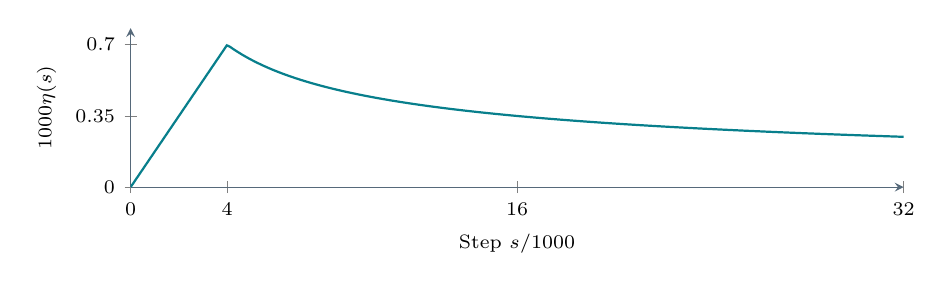
\begin{tikzpicture}
\begin{axis}[width=0.94\linewidth,height=36mm,
 xmin=0,xmax=32,ymin=0,ymax=0.78,
 xlabel={Step $s/1000$},ylabel={$1000\eta(s)$},
 xtick={0,4,16,32},ytick={0,0.35,0.7},
 tick label style={font=\scriptsize},label style={font=\scriptsize},
 axis lines=left,axis line style={muted},domain=0.001:32,samples=250]
 \addplot[accent,thick] {1000/sqrt(512)*min(1/sqrt(1000*x),1000*x/(4000*sqrt(4000)))};
\end{axis}
\end{tikzpicture}
\end{column}
\begin{column}{0.44\textwidth}
\small
For $s\leq w$, the learning rate increases linearly with $s$.
\par\vspace{2mm}
For $s\geq w$, it decreases proportionally to $s^{-1/2}$.
\par\vspace{2mm}
At $d=512$, the peak is
$\eta(w)=1/\sqrt{512\cdot4000}\approx0.000699$.
\end{column}
\end{columns}
\src{\paper, Section 5.3, Equation (3). This is a historical training choice.}
\note{The positive step convention avoids evaluating s to the power
minus one half at zero. The branches are equal when s=w, so the function
is continuous at the peak. The plot uses d=512 and displays the learning
rate multiplied by one thousand. Layer normalization placement and other
training choices can motivate different schedules in other models.}
\end{frame}

% 46
\begin{frame}[t]{Appendix H: a greedy decoding counterexample}
Consider conditional probabilities for first tokens $A$ and $B$:
\begin{center}
\begin{tabular}{@{}lcc@{}}
\toprule
Prefix & Probability of first token & Probability of EOS next \\
\midrule
$A$ & $0.60$ & $0.51$ \\
$B$ & $0.35$ & $0.99$ \\
\bottomrule
\end{tabular}
\end{center}
Other first tokens have total probability $0.05$.
\[
 p(A,\mathrm{EOS})=0.60\cdot0.51=0.306,
 \qquad p(B,\mathrm{EOS})=0.35\cdot0.99=0.3465.
\]
Greedy decoding chooses $A$ and then EOS, while the displayed
$B$ sequence has greater probability.
\src{Constructed counterexample. Finite-width beam search also has no general guarantee of finding the global optimum.}
\note{After A, the total probability of all non-EOS tokens is 0.49,
so none exceeds EOS at 0.51. Thus both greedy choices are determined.
The remaining conditional probabilities can be distributed among other
tokens. We only need one competing sequence with greater probability
to disprove global optimality. Beam search is also approximate because
discarded prefixes can later lead to a better complete sequence. Length
normalization would define a different search objective.}
\end{frame}

% 47
\begin{frame}[t]{Appendix I: rotary position embeddings}
For even $d_k$, use projected \emph{column} vectors
$\widehat q_p,\widehat k_j\in\R^{d_k\times1}$. Define
\[
 R(\phi)=\begin{bmatrix}\cos\phi&-\sin\phi\\\sin\phi&\cos\phi\end{bmatrix},
 \quad
 \mathcal R(p)=\operatorname{blockdiag}_{r=0}^{d_k/2-1}R(p\omega_r),
\]
with fixed frequencies $\omega_r=10000^{-2r/d_k}$. Rotate queries and keys:
\[
 \widetilde q_p=\mathcal R(p)\widehat q_p,\qquad
 \widetilde k_j=\mathcal R(j)\widehat k_j.
\]
Then
\[
 \widetilde q_p^{\T}\widetilde k_j
   =\widehat q_p^{\T}\mathcal R(j-p)\widehat k_j.
\]
\src{\href{https://arxiv.org/abs/2104.09864}{Su et al.}, \emph{RoFormer}. RoPE rotates projected features rather than adding the 2017 position vectors.}
\note{This slide explicitly switches to column vectors to simplify
rotation notation. Each two-dimensional rotation block satisfies
$R(a)^{\T}R(b)=R(b-a)$, giving the displayed relative-offset identity.
The content vectors still depend on the tokens, so the full score is
not solely a function of relative position. Scaling by $\sqrt{d_k}$ and
masking still apply to attention. RoPE does not by itself guarantee
accurate extrapolation to arbitrary lengths.}
\end{frame}

% 48
\begin{frame}[t]{Appendix J: review questions with answers}
\small
\begin{enumerate}
 \item \textbf{Cross-attention has $m$ queries and $n$ keys. What is the score shape?}
       $m\times n$. Normalize each row over its $n$ keys.
 \item \textbf{Which target tokens can decoder row $t=4$ use?}
       $y_1,y_2,y_3$, plus BOS and the source. Its input token is $y_3$,
       and its prediction concerns $y_4$.
 \item \textbf{How large is a stored attention array at $B=2$, $h=8$, $n=128$?}
       $2\cdot8\cdot128^2=262{,}144$ entries. With 32-bit floats,
       that is $1{,}048{,}576$ bytes, or $1$ MiB.
 \item \textbf{Does the final multi-head output lie in the convex hull of input states?}
       No general guarantee. Value projections and the output projection
       can change that set.
\end{enumerate}
\src{One MiB means $2^{20}$ bytes. The memory answer concerns one stored attention array, not an entire model.}
\note{Let the audience answer before revealing or reading the solutions.
The second answer relies on the exact row/target convention used in the
lecture. The third excludes gradients, logits, other activations, and
caches. The fourth differs from the proven single-head convex-combination
claim for already projected value vectors before dropout and output mixing.}
\end{frame}

\section{References}
% 49
\begin{frame}[t]{References: architecture and representations}
\small
\begin{thebibliography}{9}
\bibitem{vaswani}
A. Vaswani et al.\ (2017).
\emph{Attention Is All You Need}. NeurIPS.
\href{https://arxiv.org/abs/1706.03762}{arXiv:1706.03762}.
\bibitem{ba}
J. L. Ba, J. R. Kiros, and G. E. Hinton (2016).
\emph{Layer Normalization}.
\href{https://arxiv.org/abs/1607.06450}{arXiv:1607.06450}.
\bibitem{devlin}
J. Devlin et al.\ (2019).
\emph{BERT: Pre-training of Deep Bidirectional Transformers for Language Understanding}. NAACL.
\href{https://arxiv.org/abs/1810.04805}{arXiv:1810.04805}.
\bibitem{raffel}
C. Raffel et al.\ (2020).
\emph{Exploring the Limits of Transfer Learning with a Unified Text-to-Text Transformer}. JMLR.
\href{https://arxiv.org/abs/1910.10683}{arXiv:1910.10683}.
\end{thebibliography}
\note{Links point to the authors' papers. The architecture image on
slide 5 reproduces Figure 1 from Attention Is All You Need, with the
paper's attributed scholarly-reuse permission.}
\end{frame}

% 50
\begin{frame}[t]{References: variants, efficiency, and interpretation}
\footnotesize
\begin{thebibliography}{9}
\bibitem{xiong}
R. Xiong et al.\ (2020). \emph{On Layer Normalization in the Transformer Architecture}. ICML.
\href{https://proceedings.mlr.press/v119/xiong20b.html}{PMLR 119:10524--10533}.
\bibitem{dao}
T. Dao et al.\ (2022). \emph{FlashAttention: Fast and Memory-Efficient Exact Attention with IO-Awareness}. NeurIPS.
\href{https://arxiv.org/abs/2205.14135}{arXiv:2205.14135}.
\bibitem{su}
J. Su et al.\ \emph{RoFormer: Enhanced Transformer with Rotary Position Embedding}.
\href{https://arxiv.org/abs/2104.09864}{arXiv:2104.09864} (first posted 2021).
\bibitem{dosovitskiy}
A. Dosovitskiy et al.\ (2021). \emph{An Image is Worth 16x16 Words: Transformers for Image Recognition at Scale}. ICLR.
\href{https://arxiv.org/abs/2010.11929}{arXiv:2010.11929}.
\bibitem{jain}
S. Jain and B. C. Wallace (2019). \emph{Attention is not Explanation}. NAACL.
\href{https://arxiv.org/abs/1902.10186}{arXiv:1902.10186}.
\end{thebibliography}
\note{These sources describe different architectural choices and
empirical settings. Their inclusion does not imply that every Transformer
uses all of these modifications. No current leaderboard or universal
performance ranking is asserted.}
\end{frame}

\end{document}
